Ein ${\it \pi^{0}}$ zerf{\"a}llt zu $\left( 98,823\pm0,034\right)\%$ nach einer mittleren Wegl\"ange von ${\it c\tau} = 25,5$nm \cite{book:pdg} in zwei Photonen.
Als sogenannte prim\"are $\pi^{0}$ werden solche $\pi^{0}$ bezeichnet die in direkt Nukleon-Nukleon Kollisionen produziert werden.
Da der Abstand vom prim\"aren Vertex zum EMCal relativ gesehen sehr gro{\ss} ist im Vergleich zur mittleren Wegl\"ange des $\pi^{0}$, wird angenommen, dass prim\"are $\pi^{0}$ im prim\"aren Vertex zerfallen.
Der prim\"are Vertex wird mit Hilfe des ITS bestimmt, w\"ahrend Informationen \"uber Ort und Energie von Photonenkandidaten von Messungen des EMCals kommen. 
Mit diesen Informationen k{\"o}nnen prim\"are ${\pi^{0}}$ rekonstruiert werden.
\newline 
Um die invariante Masse $m_{\text{inv}}$ zu berechnen, sind die Energien $E_{\gamma1}$ und $E_{\gamma2}$ der beiden Photonenkandidaten, sowie der Zerfallswinkel $\theta_{\gamma\gamma}$ erforderlich.
\newline
Die Zahlen in den Indizes beziehen sich dabei auf die Nummerierung der beiden Photonen. Die Indizes x und y beziehen sich auf die Raumrichtungen. F{\"u}r diese gilt:
\begin{align}
m_{\text{inv}} &= \sqrt{2E_{\gamma\it{1}}E_{\gamma\it{2}}(1-\cos\left( \theta_{\gamma\gamma}\right) )} \label{eq_invmass}
\end{align}
Au{\ss}erdem kann die Aufteilung des Impulses der Photonenkandidaten bestimmt werden, die wiederum notwendig ist, um den Transversalimpuls $p_\text{T}$ des $\pi^{0}$ zu Berechnen. Es gilt:
\begin{align}
p_{T\pi^{0}} &= \sqrt{\left(p_{x1}+p_{x2}\right)^{2} +\left(p_{y1}+p_{y2}\right)^{2}} \label{eq_pt}
\end{align}
\begin{figure}[tbp] \label{figInvMassPt}
\centering
\begin{subfigure}{.5\textwidth}
	\centering
	\includegraphics[width=.95\linewidth]{hInvMass_pT_Signal.pdf}
	\caption{}
	\label{figInvMassPt_a}
\end{subfigure}%
	\begin{subfigure}{.5\textwidth}
	\centering
	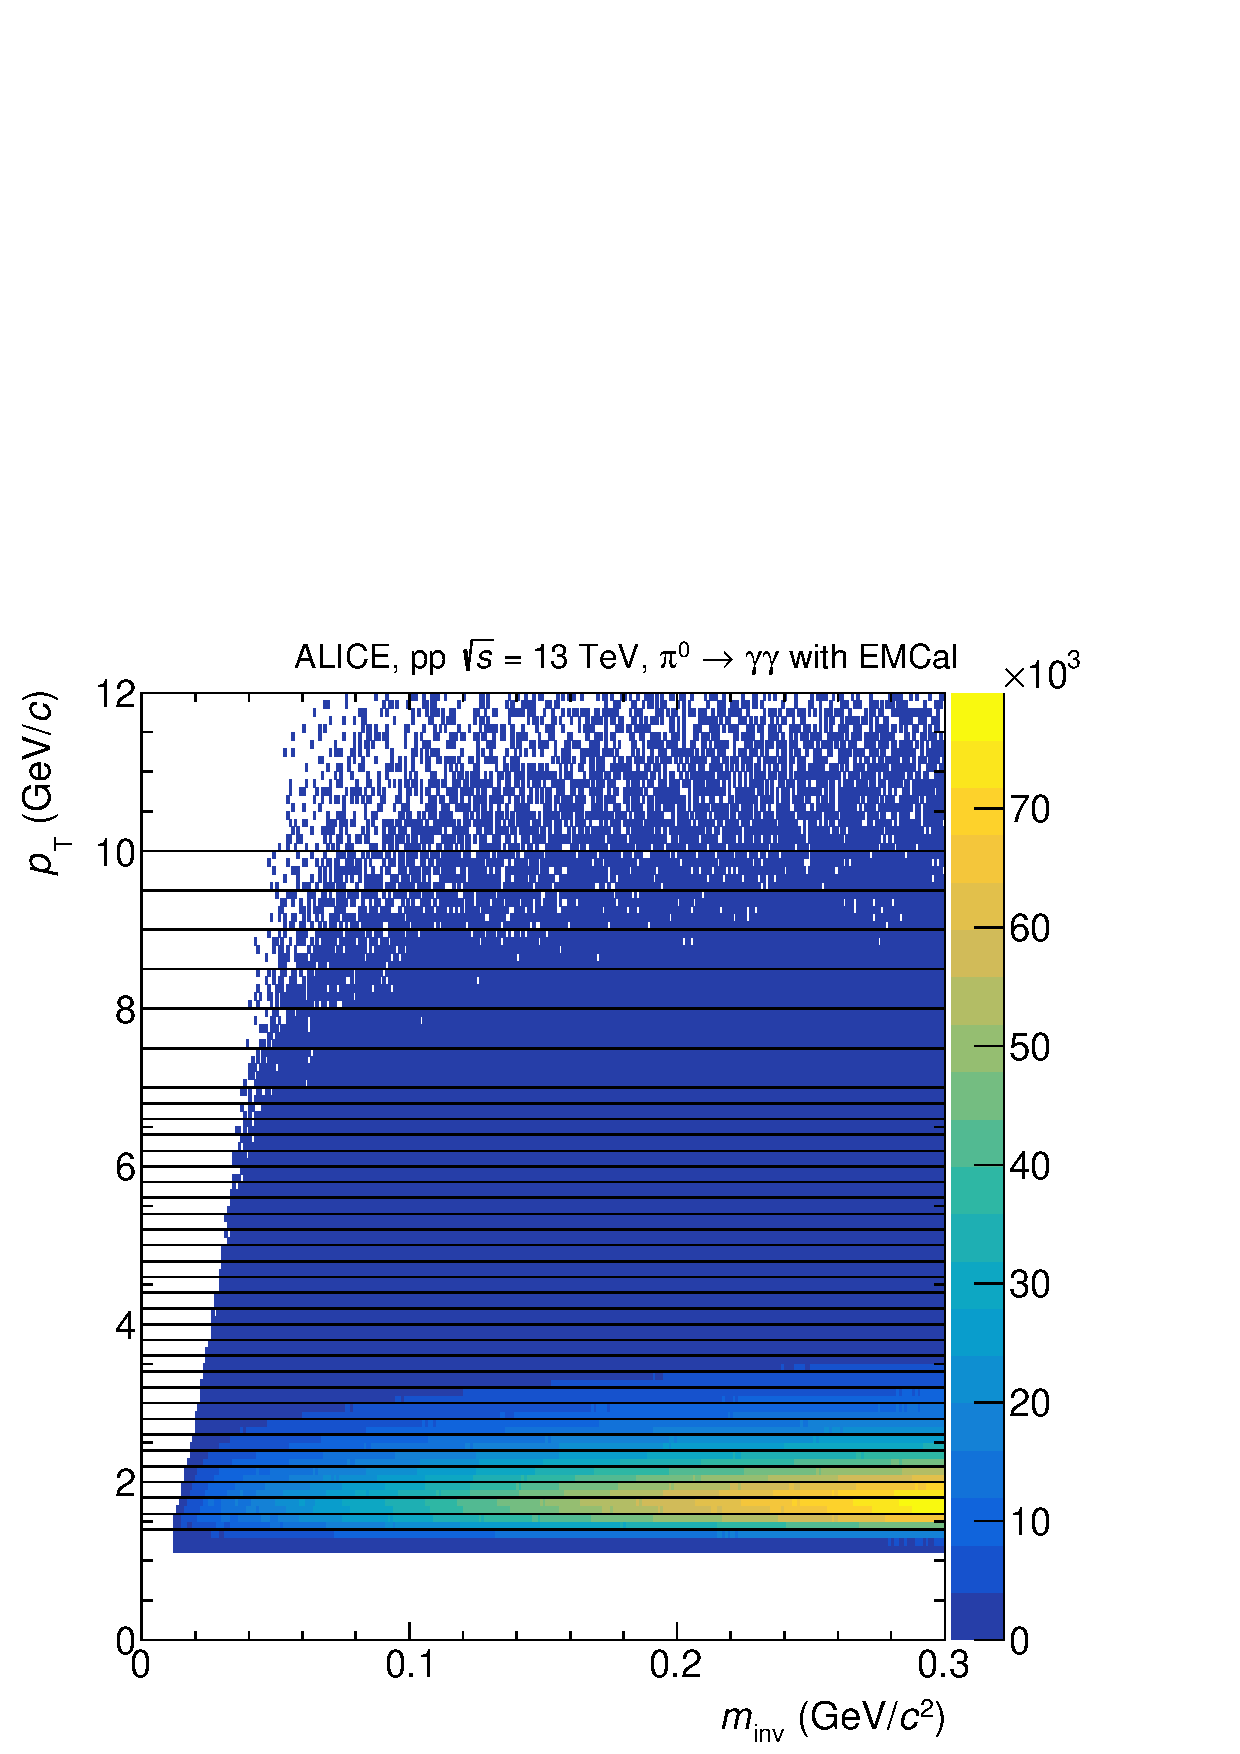
\includegraphics[width=.95\linewidth]{hInvMass_pT_Bkg.pdf}
	\caption{}
	\label{figInvMassPt_b}
\end{subfigure}
\caption{\newline{\bf (a)}: $p_\text{T}$ und $m_\text{inv}$ als Funktion von der Anzahl von rekombinierten  Cluster-Paaren aus der gleichen Kollision.
Die schwarze Linie liegt bei $m_{\text{inv}}=0,135\text{ GeV/}c^{2}$, was der $\pi^{0}$ Masse entspricht, wo eine deutliche Peakstruktur zu Erkennen ist.
\newline
{\bf (b)}: $p_\text{T}$ und $m_\text{inv}$ als Funktion von der Anzahl von rekombinierten  Cluster-Paaren aus unterschiedlichen Kollision.}
\end{figure}
\newline
Aus dem im kommenden Abschnitt \ref{s3s1s1} gew\"ahlten Datensatz werden alle m{\"o}glichen Kombinationen von zwei Photonenkandidaten aus der gleichen Kollision benutzt, um $m_{\text{inv}}$ nach Gleichung \ref{eq_invmass} zu berechnen.
Diese Methode wird auch als {\it same event} bezeichnet.
Au{\ss}erdem wird $p_{T,\pi^{0}}$ nach Gleichung \ref{eq_pt} berechnet um aus den $m_{\text{inv}}$ und $p_{T,\pi^{0}}$ Wertepaaren eine invariante Massenverteilung zu erhalten.
In Abbildung \ref{figInvMassPt_a} ist eine solche invariante Massenverteilung des Datensatzes zu sehen.
In dieser Verteilung sticht eine h{\"a}ufung der Datenpunkte bei $m_{\text{inv}}\approx 0,135\text{GeV/}c^{2}$ heraus.
Abbildung \ref{figInvMassPt_b} zeigt die invariante Massenverteilung bei der Photonenkandidaten aus unterschiedlichen Kollisionen miteinander kombiniert werden.
Diese Methode wird als {\it mixed event} bezeichnet.
\begin{figure}[tbp]
\centering
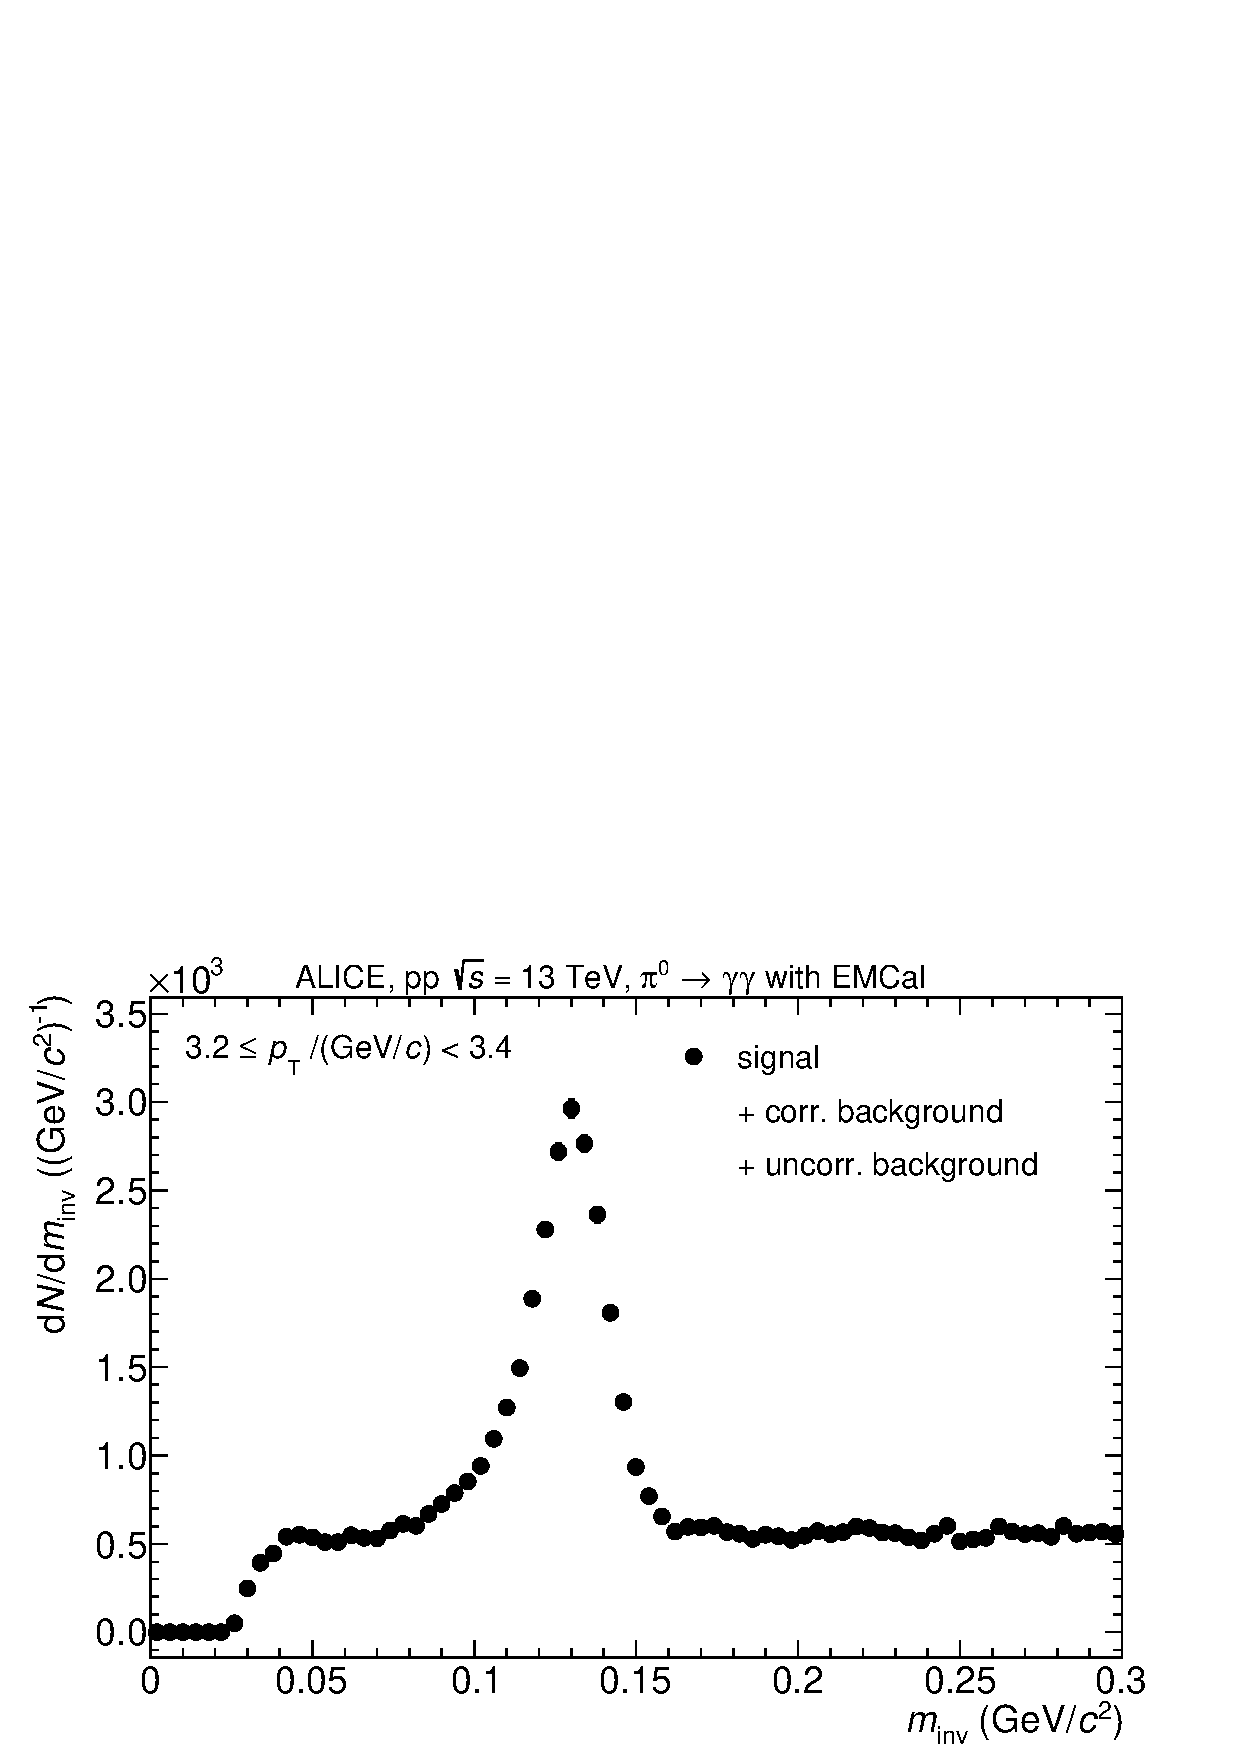
\includegraphics[width=.6\linewidth]{hSignalPlusBkg.pdf}
\caption{Projektion von Abbildung \ref{figInvMassPt_a} im $p_{\text{T}}$-Intervall (3.2 - 3.4) $(\text{GeV/}c)$. Es ist ein deutlicher Peak um $m_{\pi^{0}} \approx 0,135\text{GeV/}c^{2}$ zu erkennen, aber auch Untergrund, da das Signal zu h{\"o}heren Massen gau{\ss}f{\"o}rmig abklingen sollte. Bei $m_{\text{inv}} < m_{\pi^{0}}$ kann Signal vorliegen, das aus konvertierten Photonen besteht, weshalb eine Aussage {\"u}ber die Form, bzw. den Untergrund dort schwer m{\"o}glich ist.}
\label{figSignalPlusBkg}
\end{figure}
\newline
Um $\pi^{0}$s in einzelnen $p_{T}$-Intervallen z{\"a}hlen zu k{\"o}nnen wird die Verteilung in entsprechende Abst{\"a}nden auf die Y-Achse projiziert.
Die Intervalle werden so gew{\"a}hlt, dass sie m{\"o}glichst klein sind, w{\"a}hrend die statistischen Unsicherheiten nicht zu gro{\ss} werden.
Abbildung \ref{figSignalPlusBkg} zeigt eine Verteilungen der invarianten Masse, die aus Signal, sowie sogenanntem korrelierten und unkorrelierten Untergrund besteht.
Trotz der Untergr\"unde ist ein deutlicher Peak im Bereich der Pionenmasse von ca. 135MeV/$c^{2}$ zu erkennen.
Die Bestimmung der beiden Untergr\"unde, vor allem des korrelierten Untergrunds, ist eine wichtige Aufgabe in der Analyse von neutralen Pionen.
Das Parametrisieren einer Funktion hat sich als g\"angie Methode zur Bestimmung des korrelierten Untegr\"unds entwickelt und wird im folgenden als Standardmethode bezeichnet.
In dieser Arbeit wird der korrelierte Untergr\"und sowie das reine $\pi^{0}$-Signal mit Hilfe von sogenannten \textit{Monte Carlo Templates} bestimmt.
Die Ergebnisse der Analyse mit Hilfe von Monte Carlo Templates, sowie mit der Standardmethode werden miteinander vergleichen, um eine Aussage \"uber den m\"oglichen Nutzen von Analysen mit Hilfe von Monte Carlo Templates treffen zu k\"onnen.
Im folgenden Abschnitt wird sowohl die Standardmethode kurz, als auch die Methode mit Hilfe von Monte Carlo Templates n\"aher erl\"autert.